\documentclass[a4paper,ngerman]{scrartcl}

\usepackage{amsmath}
\usepackage{amsfonts}
\usepackage{amssymb}
\usepackage[utf8]{inputenc}
\usepackage{graphicx}
\usepackage[ngerman]{babel}
\usepackage{hyperref}
\usepackage{float}
\usepackage{caption}
\usepackage{subcaption}
\usepackage{multirow}  %for tables
\usepackage{icomma} % Handle german comma as decimal point in numbers
\usepackage{units,siunitx} % Write units with correct spacing
\usepackage{upgreek} % provide non-italic greek letters
\usepackage{url}
%\usepackage{subfig}

% Formatting of table & figure captions
\captionsetup{font={sf,footnotesize},labelfont=bf,skip=6pt}
\captionsetup[sub]{font={sf,footnotesize}} % setting for subcaptions
\sisetup{ locale = DE, % use "," as decimal point instead of "."
per-mode=fraction, % use fractions instead of ^{-1} when doing \si{... \per ...} 
exponent-product={\cdot},% used \cdot in front of 10^x
separate-uncertainty % give out uncertainty with \pm instead of in brackets
} 
\setlength{\abovecaptionskip}{6pt}
\setlength{\belowcaptionskip}{0pt}

\title{Landé-Faktor des Myons\\Versuchsvorbereitung}
\date{\today}
\author{Michel Rausch, Michael Eliachevitch}

\begin{document}

\maketitle
\tableofcontents
\newpage

\section{Einleitung}
\label{sec:einfuhrung}
% Ziel: Bestimmung der Lebensdauer und des Landé-Faktors von Myonen, 
% Myonen sinde Sekundärteilchen der kosmischen Strahlung
% wir werden ständig mit Myonen bombardiert, ohne es zu merken


\section{Theoretische Grundlagen}
\label{sec:theorie}

\subsection{Enstehung von Myonen in Luftschauern}
\label{sec:luftschauer}
% kurz schreiben, dass hochenergetische kosmische teilchen luftschauer erzeugen,
% bei denen durch hadronische wechselwirkungen geladene pionen entstehen, bei deren zerfall myonen entstehen
% vielleicht auch weglassen und erst später beim kapitel zum spin
% lebensdauer von myonen
% evtl. grober wert für den fluss von myonen aus luftschauern


\subsection{Abbremsung von Myonen in Materie}
\label{sec:wwmitmaterie}
% bei sehr hohen energien (> 1 TeV) bremmstrahlung
% bei energien im GeV Bereich Ionisation (Myonen sind 'mips' -> kleiner wirkungsquerschnitt)
% wechselwirkungen mit atomen bei niedrigen energien: 
% niederenergetische myonen wie elektronen in kern gebunden -> schneller zerfall
% antimyonen bilden kernähnliche struktur durch elektroneneinfang -> myonium

\subsection{Polarisation von Myonen}
\label{sec:polarisation}
% schwacher wechselwirkung -> vektorielle kraft und paritätsverletzung
% d.h. masselose teilchen immer linkshändig, antiteilchen rechtshändig
% da pion spin 0 hat und neutrino linkshändig ist, muss positron/antimyon auch linkshändig sein
% wegen schwacher ww wären positronen und antimyonen "lieber" rechtshändig
% da positronen kleinere masse haben als anti-muonen (faktor ~200), ist bei ihnen die rechtshändige komponente stärker unterdrückt
% analog für antineutrinos und elektronen/myuonen
% daher zerfall von piplus/piminus hauptsächlich in muonen und nicht in elektronen/positronen

% zerfall in vorwärts und rückwärtsrichtung
% myon erhält dadurch in vorwärts und rückwärtsrichtung unterschiedliche energien im laborsystem bei gleichen pionenenergien
% unterscheidbar durch polarisation



\subsection{Nachweis des Myonenzerfalls}
\label{sec:nachweis}

% die theorie hiervon kann ich auch noch nicht gut (michael)
% aber müsste nicht viel sein

\subsection{Präzession von Myonen im Magnetfeld}
\label{sec:prazission}
% gyromagnetische verhältnis gamma, landé-faktor g erklären
% präzission im magnetfeld
% am wichtigsten ist eigentlich nur folgende gleichung:
\begin{equation}
g = \frac{\gamma \hbar}{\mu_\mathrm{B}} = \frac{\hbar \omega}{\mu_\mathrm{B}\mathrm{B}}
\end{equation}

\subsection{Messprinzip}
\label{sec:messprinzip}
% zerfall von myonen erfolgt exponentialgesetz
% wie misst man präzission?
% -> angelegtes magnetfeld
% formeln...

\subsubsection*{Messung der mittleren Lebensdauer}

Die Messung startet mit der Registrierung der Abbremsung eines Myons im Detektor. Durch den Zerfall entsteht ein Positron, dessen Auftreten die Messung stoppt. Da es sich um einen Zerfall handelt, kann man für viele beobachtete Myonen ein Exponentialgesetz ansetzen:

\begin{equation}
\label{eqn:messprinzip-zerfall}
N(T) = N_0 \cdot exp(-t / \tau) .
\end{equation} 
	
$N_0$ ist die Gesamtzahl der im Detektor gestoppten Myonen während der Messzeit, $N$ die Anzahl der beobachteten Zerfälle.
Die mittlere Lebensdauer $\tau$ kann man bestimmen, auch ohne die Energie und Richtung der Myonen zu betrachten. 

\subsubsection*{Messung der Präzessionsfrequenz}


Über das Stopptarget wird ein Magnetfeld transversal zur Einfallsrichtung der Myonen gelegt, in diese präzedieren.
Indem nur in eine bestimmte Richtung emittierte Positronen gemessen werden, ist die Zählrate mit der Präzessionsfrequenz moduliert. Ist der Spin der Myonen antiparallel zur Richtung, ist er am geringsten, bei parallel gerichtetem am höchsten.


Gleichungen und \ref{eqn:messprinzip-zerfall}

%!!!!!!!!!!!!!!!!!!!!!! Gleichungsnummer einfügen, 7-116 aus BB.

lassen sich zusammenfassen zu

\begin{equation}
N(t) = K \cdot exp(- \frac{t}{\tau}) \cdot \left[ 1 + \overline{A} \cdot cos(\omega t + \delta) \right] .
\end{equation}

Die Exponentialfunktion entstammt dem Zerfallsgesetz aus Gleichung \ref{eqn:messprinzip-zerfall}, der Term in der eckigen Klammer beschreibt die Modulation durch Präzession.
$\overline{A}$ ist die, über die Geometrie des Detektors gemittelte, Asymmetrie. Diese ist aufgrund der Depolarisation der $\mu^{+}$ zeitabhängig und folgt einem Exponentialgesetz

\begin{equation}
\overline{A} = \overline{A}_0 \cdot exp(- \frac{t}{ T_R }) .
\end{equation}

In Kupfer kann sie jedoch als konstant angenommen werden. $T_R$ bezeichnet die Relaxationszeit.
	
\clearpage

\section{Versuchsaufbau und Durchführung}
% von oben nach unten: Szinti 1, Szinti 2, Kupferabsorber in Magnetfeld, Szinti 3
% Koinzindenz und Veto-Schaltung erklären: 
% D.h. Wir nehmen nur die Ereignisse, wo 1 und 2 gleichzeitig ausschlagen (Koinzindenz) und 3 NICHT ausschlägt (Veto bzw Antikoinzindenz)
% erklären was ein diskriminator in der analog-digitalwandlung ist und wie die schwelle (trigger) eingestellt werden muss:
% trigger muss so sein, dass untergrund unterdrückt wird und man nur hauptsignal sieht
% zu hoher trigger verringer unnötig statistik
% trigger für veto (szinti 3) lieber etwas niedriger als zu hoch, damit man keine falschen ereignisse aufnimmt
% was ist ein TAC (zeit-amplituden-converter) und zeiteichung ?

In Abbildung \ref{fig:aufbau_skizze} ist eine Skizze des Versuchsaufbaus gezeigt. Drei Szintillatorplatten, mit einer Dicke von $\SI{2.5}{cm}$, sind waagerecht übereinandergelegt. Zwischen dem zweiten und dritten befindet sich eine ebenso dicke Kupferplatte, welches die $\mu^{+}$ stoppt. 
Signale aus den Szintillatoren werden mit einem Photomultiplier (PM) verstärkt und in die Koinzidenz geschickt.
Ein gestopptes Myon hat die Signatur $1 + 2 + \overline{3}$, also eine Koinzidenz der oberen Szintillatoren und eine Antikoinzidenz des unteren. Damit wird die Messsung begonnen. Die Messung wird beendet, wenn ein Positron detektiert wird. Dieses kann in Richtung des Szintillators 2, oder 3 emittiert werden. Das Stoppsignal auszusenden, wenn eines der beiden Szintillatoren ein Signal aussendet ist jedoch nicht optimal, da zufällige Stopps aufgrund von Hintergrundstrahlung auftreten. Am besten eignet sich eine Signatur $1 + 2 + \overline{3}$. Die Zählrate ist hier jedoch abgeschwächt.  


\begin{figure}[tb!]
  \centering
  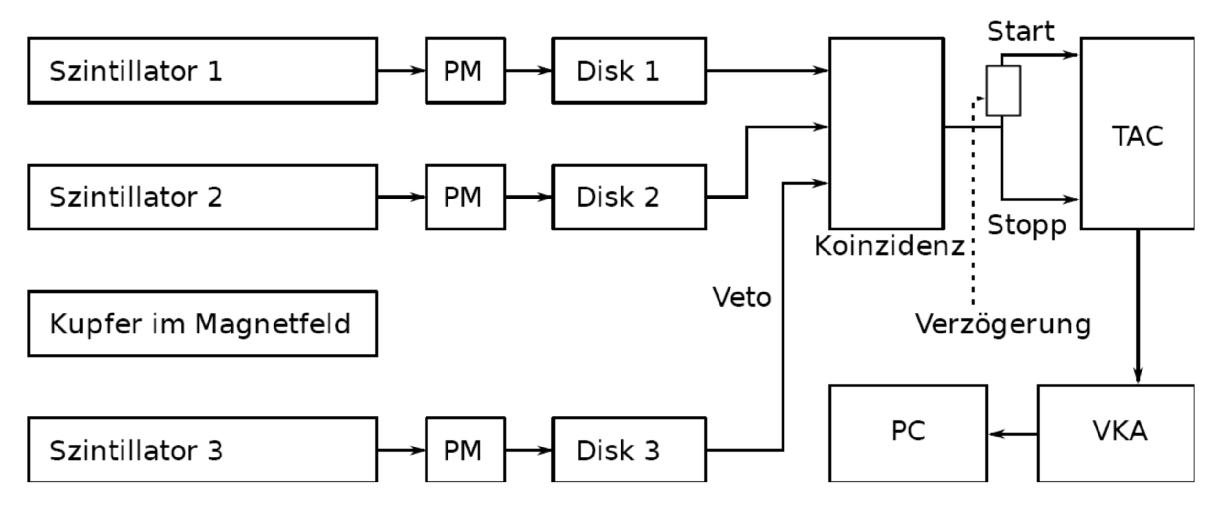
\includegraphics[width=0.8\textwidth]{abbildungen/aufbau_skizze.png}
  \caption{\textbf{Skizze des Versuchsaufbaus.} 
  \\ 
  Drei Kunstoffszintillatoren und eine Kupferplatte mit einer Dicke von jeweils $\SI{2.5}{cm}$ sind übereinander angeordnet. Die Kupferplatte befindet sich zwischen dem 2. und 3. Szintillator. Das Signal aus den Szintillatoren wird mit Photomultpliern (\textbf{PM}) verstärkt. Bei den definierten Signatur wird von der Koinzidenz ein Signal für den Start, bzw. Stopp der Messung gegeben. Das Startsignal wird um einige Nanosekunden verzögert, damit der Time to Amplitude Converter (\textbf{TAC}) das Signal verarbeiten kann. Über einen Vielkanalanalysator (\textbf{VKA}) wird das Signal an einem Rechner (\textbf{PC}) analysiert.
  \\Quelle: [\ref{ref:bb}]}
  \label{fig:aufbau_skizze}
\end{figure}


\subsection{Zusätzliche Aufgaben}

\begin{enumerate}[(a)]
\item Einstellung der Schwellen an den Diskriminatoren
\item Zeiteichung des Zeit-zu-Amplituden-Konverters (TAC)
\end{enumerate}



\clearpage
\section{Quellen}
\begin{enumerate}
\item \emph{Einführung in das Kernphysikalische Praktikum} von F. K. Schmidt, 
  Überarbeitung von J. Wolf, Ausgabe September 2009 \label{ref:bb}
\end{enumerate}



\end{document}
